\documentclass{article}
\usepackage{tikz}
\pagestyle{empty}
\begin{document}
\usetikzlibrary{arrows}
\usetikzlibrary{shapes}
\usetikzlibrary{snakes}
\usetikzlibrary{patterns}


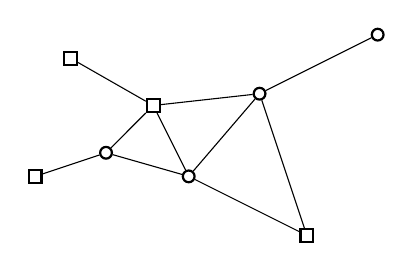
\begin{tikzpicture}[scale=1.5]
  \tikzstyle{terminal} = [draw, thick, minimum size=0.2, inner sep=2.3pt];
  \tikzstyle{steiner} = [circle, draw, thick, minimum size=0.2, inner sep=1.5pt];

  \node[terminal] (t1) at (1.2,1) {};
  \node[terminal] (t2) at (3.5,0.5) {};
  \node[terminal] (t3) at (1.5,2.0) {};
  \node[steiner] (t4) at (4.1,2.2) {};

  \node[steiner] (s1) at (1.8,1.2) {};
  \node[steiner] (s2) at (3.1,1.7) {};
  \node[steiner] (s3) at (2.5,1.0) {};
  \node[terminal] (s4) at (2.2,1.6) {};

  \draw (t1) -- (s1);
  \draw (t2) -- (s2);
  \draw (t2) -- (s3);
  \draw (t3) -- (s4);
  \draw (t4) -- (s2);

  \draw (s1) -- (s4);
  \draw (s4) -- (s3);
  \draw (s3) -- (s2);
  \draw (s2) -- (s4);
  \draw (s1) -- (s3);

\end{tikzpicture}
\end{document}